\section{Volume}{}{}\label{sec:volume}
Now that we have seen how to compute certain areas by using integration; we will now look into how some
volumes may also be computed by evaluating an integral. Generally, the
volumes that we can compute this way have cross-sections that are easy
to describe.

The volume of a general right cylinder, as shown in Figure \ref{fig:cross1} has a simple calculation, it is  equal to base $\times$ height. \hfill\null

\begin{figure}[H]
\centering
\includegraphics[width=0.2\textwidth]{/figures/figcross1_3D}
\caption{The volume of a general right cylinder}
\label{fig:cross1}
\end{figure}


\noindent We can use this fact as the building block in finding volumes of a variety of shapes.

Given an arbitrary solid, we can \textit{approximate} its volume by cutting it into $n$  thin slices. When the slices are thin, each slice can be approximated well by a general right cylinder. Thus the volume of each slice is approximately its cross-sectional area $\times$ thickness. (These slices are the differential elements.)

By orienting a solid along the $x$-axis, we can let $A(x_i)$ represent the cross-sectional area
of the $i\,^\text{th}$ slice, and let $\dx_i$ represent the thickness of this slice (the thickness is a small change in $x$). The total volume of the solid is approximately:
	\begin{align*} \text{Volume} &\approx \sum_{i=1}^n \Big[\text{Area}\ \times\ \text{thickness}\Big] \\
			&= \sum_{i=1}^n A(x_i)\dx_i.
	\end{align*}
	
Recognize that this is a Riemann Sum. By taking a limit (as the thickness of the slices goes to 0) we can find the volume exactly. 

\begin{theorem}{Volume By Cross-Sectional Area}{volume_by_cross_section}
{The volume $V$ of a solid, oriented along the $x$-axis with cross-sectional area $A(x)$ from $x=a$ to $x=b$, is \index{integration!volume!cross-sectional area}
$$V = \int_a^b A(x)\ dx.$$
}
\end{theorem}

\begin{example}{Finding the volume of a solid}{ex_disk0}
{
Find the volume of a pyramid with a square base of side length $ 10 $ cm and a height of $ 5 $ cm.}
\end{example}


\begin{solution}
{There are many ways to ``orient'' the pyramid along the $x$-axis; Figure \ref{fig:disk0} gives one such way, with the pointed top of the pyramid at the origin and the $x$-axis going through the center of the base.

\begin{figure}[H]
\centering
\includegraphics[width=0.35\textwidth]{figures/figcross_area1}
\caption{Orienting a pyramid along the $x$-axis in Example \ref{ex_disk0}.}
\label{fig:disk0}
\end{figure}


Each cross section of the pyramid is a square; this is a sample differential element. To determine its area $A(x)$, we need to determine the side lengths of the square.

When $x=5$, the square has side length $ 10 $; when $x=0$, the square has side length $ 0 $. Since the edges of the pyramid are lines, it is easy to figure that each cross-sectional square sitting above $ x $, has side length $2x$, giving $A(x) = (2x)^2=4x^2$. % 

If one were to cut a slice out of the pyramid at $x=3$, as shown in Figure \ref{fig:disk0a}, one would have a shape with square bottom and top with sloped sides. If the slice were thin, both the bottom and top squares would have sides lengths of about 6, and thus the cross--sectional area of the bottom and top would be about 36in$^2$. Letting $\Delta x_i$ represent the thickness of the slice, the volume of this slice would then be about $36\Delta x_i$in$^3$. 

\begin{figure}
\centering
\includegraphics[width=0.6\textwidth]{figures/figcross_area1a_3D}
\caption{Cutting a slice in the pyramid in Example \ref{ex_disk0} at $x=3$.}
\label{fig:disk0a}
\end{figure}



Cutting the pyramid into $n$ slices divides the total volume into $n$ equally--spaced smaller pieces, each with volume $(2x_i)^2\Delta x$, where $x_i$ is the approximate location of the slice along the $x$-axis and $\Delta x$ represents the thickness of each slice. One can approximate total volume of the pyramid by summing up the volumes of these slices:
$$\text{Approximate volume } = \sum_{i=1}^n (2x_i)^2\Delta x.$$
Taking the limit as $n\to\infty$ gives the actual volume of the pyramid; recognizing this sum as a Riemann Sum allows us to find the exact answer using a definite integral, matching the definite integral given by Theorem \ref{thm:volume_by_cross_section}.

We have 
\begin{align*} V &= \lim_{n\to\infty} \sum_{i=1}^n (2x_i)^2\Delta x\\
							&= \int_0^5 4x^2\ dx\\
				&= \frac43x^3\Big|_0^5 \\
				&=\frac{500}{3}\ \text{cm}^3 \approx 166.67\ \text{cm}^3.
\end{align*}
We can check our work by consulting the general equation for the volume of a pyramid (see the back cover under ``Volume of A General Cone''): 

\hfill $\frac13\times \text{area of base}\times \text{height}$.\hfill \null

\noindent Certainly, using this formula from geometry is faster than our new method, but the calculus--based method can be applied to much more than just cones.
}
\end{solution}

\begin{example}{Volume of an Object}{Volume of an Object}
The base of a solid is the region between $\ds f(x)=x^2-1$ and
$\ds g(x)=-x^2+1$, and its cross-sections perpendicular to the $x$-axis 
are equilateral triangles, as indicated in
Figure~\xrefn{fig:triangular cross-sections}.
%\texonly
The solid has been truncated to show a triangular
cross-section above $x=1/2$.
%\endtexonly
Find the volume of the solid.
\end{example}

\figure[H]
%\texonly
\centerline{\vbox{\beginpicture
\normalgraphs
%\ninepoint
\setcoordinatesystem units <3truecm,3truecm>
\setplotarea x from -1.1 to 1.1, y from -1.1 to 1.1
\put {\hbox{\epsfxsize6truecm\epsfbox{images/triangular_solid.eps}}} at 3 0
\axis bottom shiftedto y=0 ticks withvalues {$-1\quad$} {$1$} / at -1 1 / /
\axis left shiftedto x=0 ticks withvalues {$-1\quad$} {$1\quad$} / at -1 1 / /
\plot
-1.000 0.000 -0.900 -0.190 -0.800 -0.360 -0.700 -0.510 -0.600 -0.640 
-0.500 -0.750 -0.400 -0.840 -0.300 -0.910 -0.200 -0.960 -0.100 -0.990 
0.000 -1.000 0.100 -0.990 0.200 -0.960 0.300 -0.910 0.400 -0.840 
0.500 -0.750 0.600 -0.640 0.700 -0.510 0.800 -0.360 0.900 -0.190 
1.000 0.000 /
\plot
-1.000 0.000 -0.900 0.190 -0.800 0.360 -0.700 0.510 -0.600 0.640 
-0.500 0.750 -0.400 0.840 -0.300 0.910 -0.200 0.960 -0.100 0.990 
0.000 1.000 0.100 0.990 0.200 0.960 0.300 0.910 0.400 0.840 
0.500 0.750 0.600 0.640 0.700 0.510 0.800 0.360 0.900 0.190 
1.000 0.000 /
\endpicture}}
%\begincaption
%{Solid with equilateral triangles as cross-sections.
%(\expandafter\url\expandafter{\liveurl jmol_triangular_x_sections}%
%AP\endurl)}
%%(\expandafter\url\expandafter{\sageurl solid_with_triangular_x-sections}%
%%AP\endurl)}
%\endcaption
%\endtexonly
%\figrdef{fig:triangular cross-sections}
%\htmlfigure{Integration_applications-volume_equilateral_x_sections.html}
%\htmlonly
\caption
{Solid with equilateral triangles as cross-sections.\label{fig:triangular cross-sections}}
%You can download the <a href="http://www.whitman.edu/mathematics/calculus/live/sage/solid_with_triangular_x-sections/solid_with_triangular_x-sections.sws">Sage worksheet</a>
%for this plot and upload it to your own sage account.
%\endcaption
%\endhtmlonly
\endfigure

\begin{solution}
A cross-section taken at say $ x_i$ on the $x$-axis is a triangle with
base $\ds 2(1-x_i^2)$ and height $\ds \sqrt3(1-x_i^2)$, so the area of the
cross-section is 
$$
 A(x_i) {1\over2}(\hbox{base})(\hbox{height})=
  (1-x_i^2)\sqrt3(1-x_i^2),
$$
and the volume of a thin ``slab'' is then
$$(1-x_i^2)\sqrt3(1-x_i^2)\Delta x.$$
Thus the total volume is 
$$\int_{-1}^1 A(x) \; dx = \int_{-1}^1 \sqrt3(1-x^2)^2\,dx={16\over15}\sqrt3.$$
\vskip-10pt
\end{solution}
%
%
%
%
An important special case of Theorem \ref{thm:volume_by_cross_section} is when the solid is a \textbf{solid of revolution}, that is, when the solid is formed by rotating a shape around some axis of rotation.

Start with a function $y=f(x)$ from $x=a$ to $x=b$. Revolving this curve about a horizontal axis creates a three-dimensional solid whose cross sections are disks (thin circles). Let $R(x)$ represent the radius of the cross-sectional disk at $x$; the area of this disk is $\pi R(x)^2$. Applying Theorem \ref{thm:volume_by_cross_section} gives the Disk Method.

For example, in Figure~\ref{fig:solid of rotation} 
we see a plane region under a curve and between two
vertical lines; then the result of rotating this around the $\ds x$-axis, and
a typical circular cross-section is a circle.

\figure[H]
%\texonly
\centerline{
\vbox{\hbox{\hfill\raise53pt\vbox{
\beginpicture
\normalgraphs
%\ninepoint
\setcoordinatesystem units <5.5truemm,5.5truemm>
\setplotarea x from 0 to 8, y from -4 to 4
\axis left /
\axis bottom shiftedto y=0 / 
\putrule from 1 0 to 1 4 
\putrule from 6 0 to 6 3
\plot 1 4 1.150 3.546 
1.312 3.125 1.475 2.772 1.638 2.484 1.800 2.255 1.962 2.082 
2.125 1.961 2.288 1.886 2.450 1.854 2.612 1.859 2.775 1.898 
2.938 1.967 3.100 2.060 3.262 2.174 3.425 2.303 3.588 2.444 
3.750 2.593 3.912 2.744 4.075 2.894 4.238 3.037 4.400 3.170 
4.562 3.289 4.725 3.388 4.888 3.464 5.050 3.511 5.212 3.527 
5.375 3.505 5.538 3.443 5.700 3.334 5.862 3.176 6.025 2.964 /
\endpicture}
\quad\epsfxsize3.8cm\epsfbox{images/rotated_surface.eps}
\quad\epsfxsize3.8cm\epsfbox{images/one_disk.eps}
\hfill}\vglue-0pt}}
\caption{\label{fig:solid of rotation} A solid of rotation.}
\endfigure

\begin{formulabox}[The Disk Method \label{idea:disk_method}]
{Let a solid be formed by revolving the curve $y=f(x)$ from $x=a$ to $x=b$ around a horizontal axis, and let $R(x)$ be the radius of the cross-sectional disk at $x$. The volume of the solid is
\index{integration!volume!Disk Method}\index{Disk Method}
$$V = \pi \int_a^b R(x)^2\ dx.$$
}
\end{formulabox}


Of course a real ``slice'' of this figure will not have straight
sides, but we can approximate the volume of the slice by a cylinder or
disk with circular top and bottom and straight sides; the volume of
this disk will have the form $\ds \pi r^2\Delta x$. As long as we can
write $r$ in terms of $x$ we can compute the volume by an integral.

\begin{example}{Finding volume using the Disk Method}{ex_disk1}{
Find the volume of the solid formed by revolving the curve $y=1/x$, from $x=1$ to $x=2$, around the $x$-axis.}
\end{example}

%
\begin{solution}
{A sketch can help us understand this problem. In Figure \ref{fig:disk1}(a) the curve $y=1/x$ is sketched along with the differential element -- a disk -- at $x$ with radius $R(x)=1/x$. In Figure \ref{fig:disk1} (b) the whole solid is pictured, along with the differential element. 

The volume of the differential element shown in part (a) of the figure is approximately $\pi R(x_i)^2\Delta x$, where $R(x_i)$ is the radius of the disk shown and $\Delta x$ is the thickness of that slice. The radius $R(x_i)$ is the distance from the $x$-axis to the curve, hence $R(x_i) = 1/x_i$.
	



\begin{figure}
	\centering
	\begin{subfigure}[t]{0.5\textwidth}
		\includegraphics[width=\textwidth]{figures/figdisk1}
        \label{fig:disk1}
        \caption{} 
    \end{subfigure}% 
    \begin{subfigure}[t]{0.5\textwidth}
    \includegraphics[width=\textwidth]{figures/figdisk1b}
        \label{fig:disk1b}
        \caption{}    
    \end{subfigure} 
    \caption{Sketching a solid in Example \ref{exa:ex_disk1} \label{fig:disk}}
\end{figure}


%\mtable{.5}{Sketching a solid in Example \ref{ex_disk1}.}{fig:disk1}{%
%		\begin{tabular}{c} %
%		\myincludegraphicsthree{width=110pt,3Dmenu,activate=onclick,deactivate=onclick,
%3Droll=126.0060482236849,
%3Dortho=0.004875946324318647,
%3Dc2c=0.44462037086486816 0.39410829544067383 0.8043577671051025,
%3Dcoo=67.21983337402344 3.5258262157440186 -29.566415786743164,
%3Droo=150.00000160608386,
%3Dlights=Headlamp,add3Djscript=asylabels.js}{}{figures/figdisk1}\\
%%\myincludegraphics{figures/figdisk1} \\
%		(a) \\
%		\myincludegraphicsthree{width=110pt,3Dmenu,activate=onclick,deactivate=onclick,
%3Droll=126.0060482236849,
%3Dortho=0.004875946324318647,
%3Dc2c=0.44462037086486816 0.39410829544067383 0.8043577671051025,
%3Dcoo=67.21983337402344 3.5258262157440186 -29.566415786743164,
%3Droo=150.00000160608386,
%3Dlights=Headlamp,add3Djscript=asylabels.js}{}{figures/figdisk1b}\\
%%\myincludegraphics{figures/figdisk1b} \\
%		(b) 
%		\end{tabular}
%}
Slicing the solid into $n$ equally--spaced slices, we can approximate the total volume by adding up the approximate volume of each slice:
$$\text{Approximate volume } = \sum_{i=1}^n \pi \left(\frac1{x_i}\right)^2\Delta x.$$

Taking the limit of the above sum as $n\to\infty$ gives the actual volume; recognizing this sum as a Riemann sum allows us to evaluate the limit with a definite integral, which matches the formula given in Key Idea \ref{idea:disk_method}:

%Using Key Idea \ref{idea:disk_method}, we have 
\begin{align*}
	V = \lim_{n\to\infty}\sum_{i=1}^n \pi \left(\frac1{x_i}\right)^2\Delta x
		= \pi\int_1^2 \left(\frac1x\right)^2\ dx 
		= \pi\int_1^2 \frac1{x^2}\ dx
		&= \pi\left[-\frac1x\right]\Big|_1^2 \\
		&= \pi \left[-\frac12 - \left(-1\right)\right] \\
		&= \frac{\pi}{2}\ \text{units}^3.
\end{align*}

\vskip-\baselineskip
}
\end{solution}



\textbf{Note:} While Key Idea \ref{idea:disk_method} is given in terms of functions of $x$, the principle involved can be applied to functions of $y$ when the axis of rotation is vertical, not horizontal. We demonstrate this in the next example.\\

\clearpage

\begin{example}{Finding volume using the Disk Method}{ex_disk2}{
	Find the volume of the solid formed by revolving the curve $\ds y=\frac1x$, from $x=1$ to $x=2$, about the $y$-axis.}	
\end{example}

\begin{solution}
{Since the axis of rotation is vertical, we need to convert the function into a function of $y$ and convert the $x$-bounds to $y$-bounds. Since $y=1/x$ defines the curve, we rewrite it as $x=1/y$. The bound $x=1$ corresponds to the $y$-bound $y=1$, and the bound $x=2$ corresponds to the $y$-bound $y=1/2$. 
	
Thus we are rotating the curve $x=1/y$, from $y=1/2$ to $y=1$ about the $y$-axis to form a solid. The curve and sample differential element are sketched in Figure \ref{fig:disk2} (a), with a full sketch of the solid in Figure \ref{fig:disk2} (b).
	
	


\begin{figure}[H]
	\centering
	\begin{subfigure}[t]{0.5\textwidth}
		\includegraphics[width=\textwidth]{figures/figdisk1a}
		\label{fig:disk1a}
		\caption{} 
	\end{subfigure}%
	~ 
	\begin{subfigure}[t]{0.5\textwidth}    
		\includegraphics[width=\textwidth]{figures/figdisk2a}
		\label{fig:disk2a}
		\caption{}    
	\end{subfigure} 
	\caption{Sketching a solid in Example \ref{exa:ex_disk2}. \label{fig:disk2}}
\end{figure}	



	We integrate to find the volume:
\[
V = \pi\int_{1/2}^1 \frac{1}{y^2}\ dy  = -\frac{\pi}y\Big|_{1/2}^1  = \pi\ \text{units}^3.
\]
}
	
\end{solution}	


\begin{example}{Volume of a Right Circular Cone}{Volume of a Right Circular Cone}\label{Volume of a Right Circular Cone}
Find the volume of a right circular cone with base radius 10 and
height 20. (A right circular cone is one with a circular base and with
the tip of the cone directly over the center of the base.)
\end{example}

\begin{solution}
We can view this cone as produced by the rotation of the line $y=x/2$ between $ x=0 $ and $ x= 20 $ rotated about the $x$-axis, as indicated in
figure~\ref{fig:line to cone}.





% rotated around the y-axis
%\begin{tikzpicture}
% \begin{axis}[view={60}{30}]
%  \addplot3[surf,shader=flat,
%  samples=20,
%  domain=1:2,y domain=0:2*pi,
%  z buffer=sort]
%  ({x * cos(deg(y))}, {x * sin(deg(y))}, {1/x});
% \end{axis}
%\end{tikzpicture}

% rotated around the x-axis

\begin{figure}[H]
\begin{tikzpicture}[scale=.7,/pgf/declare function={f=(x/2);}]
\begin{axis}[
        xmin=0,xmax=20,ymin=0,ymax=10,
    domain=0:20,
    samples=10,
    y=0.4cm,
    x=0.4cm,
    axis lines=middle
]
\addplot [thick, blue, ,name path=A] {f}  node[midway, above, sloped] {$f(x) =x/2$};
 \addplot [draw=none,name path=B] {0};     % “fictional” curve
  \addplot [blue!50] fill between[of = A and B,soft clip={domain=0:20}]; % filling
  %\draw (axis cs:6,6) node { $\ds y=\frac{x}{2}$};
\end{axis}
\end{tikzpicture}
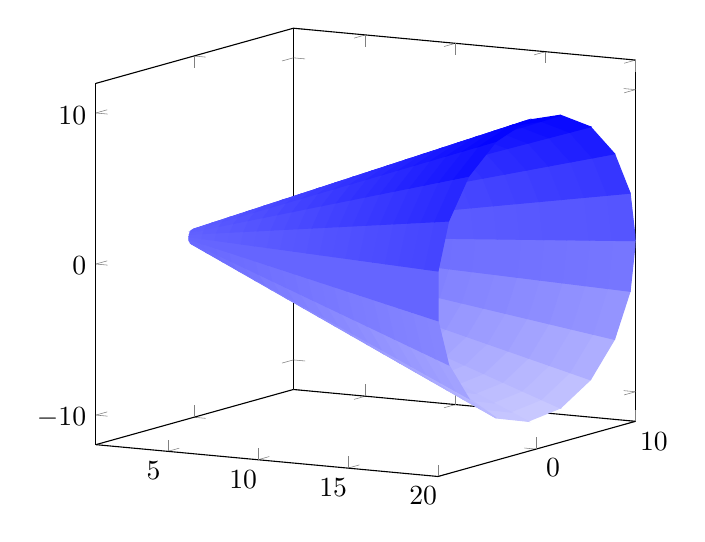
\begin{tikzpicture}
 \begin{axis}[view={30}{10}, colormap={custom}{color(0)=(blue!20) color(1)=(blue)}]
  \addplot3[surf,shader=flat,
  samples=20,
  domain=1:20,y domain=0:2*pi,
  z buffer=sort]
  (x,{(x/2) * cos(deg(y))}, {(x/2) * sin(deg(y))});
 \end{axis}
\end{tikzpicture}
\caption{\label{fig:line to cone}
A region that generates a cone; approximating the volume
by circular disks.}
\end{figure}



%\figure[H]
%%\texonly
%\centerline{\vbox{\beginpicture
%\normalgraphs
%%\ninepoint
%\setcoordinatesystem units <0.25truecm,0.25truecm>
%\setplotarea x from 0 to 20, y from 0 to 10
%\axis bottom shiftedto y=0 ticks withvalues {$0$} {$20$} / at 0 20 / /
%\put {\hbox{\epsfxsize6cm\epsfbox{images/cone.eps}}} at 40 5
%\plot 0 0 20 10 /
%\putrule from 20 0 to 20 10
%\endpicture}}
%\caption{\label{fig:line to cone}
%A region that generates a cone; approximating the volume
%by circular disks.}
%%(\expandafter\url\expandafter{\liveurl cone.html}%
%%AP\endurl)
%%\endcaption
%%\endtexonly
%%\figrdef{fig:line to cone}
%%\htmlfigure{Integration_applications-volume_of_cone.html}
%%\begincaption
%%Approximating the volume of a cone
%%by circular disks.
%%\endcaption
%\endfigure

At a particular point on the $x$-axis, say $\ds x_i$, the radius of the
resulting cone is the $y$-coordinate of the corresponding point on the
line, namely $\ds y_i=x_i/2$. Thus the total volume is approximately
$$\sum_{i=0}^{n-1} \pi (x_i/2)^2\,dx$$
and the exact volume is
$$
  \int_0^{20} \pi
  {x^2\over4}\,dx={\pi\over4}{20^3\over3}={2000\pi\over3}.
$$ 
Note that we can instead do the calculation with a generic height and
radius: 
$$
  \int_0^{h} \pi{r^2\over h^2}x^2\,dx
  ={\pi r^2\over h^2}{h^3\over3}={\pi r^2h\over3},
$$ 
giving us the usual formula for the volume of a cone.
\end{solution}


%
We can also compute the volume of solids of revolution that have a hole in the centre. The general principle is simple: compute the volume of the solid irrespective of the hole, then subtract the volume of the hole. If the outside radius of the solid is $R(x)$ and the inside radius (defining the hole) is $r(x)$, then the volume is 
$$V = \pi\int_a^b R(x)^2 \ dx - \pi\int_a^b r(x)^2\ dx = \pi\int_a^b \left(R(x)^2-r(x)^2\right)\ dx.$$



\begin{figure}[H]
	\centering
	\begin{subfigure}[t]{0.5\textwidth}
		\includegraphics[width=\textwidth]{figures/figwasher_idea_a}
		%\label{fig:disk1a}
		\caption{} 
	\end{subfigure}%
	~ 
	\begin{subfigure}[t]{0.5\textwidth}    
		\includegraphics[width=\textwidth]{figures/figwasher_idea_b}
		%\label{fig:disk2a}
		\caption{}    
	\end{subfigure} 
	\caption{Establishing the Washer Method; see also Figure \ref{fig:washeridea_b}. \label{fig:washeridea}}
\end{figure}	




One can generate a solid of revolution with a hole in the middle by revolving a region about an axis. Consider Figure \ref{fig:washeridea}(a), where a region is sketched along with a dashed, horizontal axis of rotation. By rotating the region about the axis, a solid is formed as sketched in Figure \ref{fig:washeridea}(b). The outside of the solid has radius $R(x)$, whereas the inside has radius $r(x)$. Each cross section of this solid will be a washer (a disk with a hole in the center) as sketched in Figure \ref{fig:washeridea_b}.	This leads us to the Washer Method.


\begin{figure}[H]
\centering
\includegraphics[width=0.65\textwidth]{figures/figwasher_idea_c}
\caption{Establishing the Washer Method; see also Figure \ref{fig:washeridea}.}
\label{fig:washeridea_b}
\end{figure}

%\mfigurethree{width=125pt,3Dmenu,activate=onclick,deactivate=onclick,
%3Droll=96.94265756936434,
%3Dortho=0.005309578496962786,
%3Dc2c=0.547386884689331 0.07732175290584564 0.833299994468689,
%3Dcoo=64.78053283691406 10.129053115844727 -47.566162109375,
%3Droo=149.99999789136484,
%3Dlights=Headlamp,add3Djscript=asylabels.js}{}{.8}{Establishing the Washer Method; see also Figure \ref{fig:washeridea}.}{fig:washeridea_b}{figures/figwasher_idea_c}


\begin{formulabox}[The Washer Method \label{idea:washermethod} ]
{Let a region bounded by $y=f(x)$, $y=g(x)$, $x=a$ and $x=b$ be rotated about a horizontal axis that does not intersect the region, forming a solid. Each cross section at $x$ will be a washer with outside radius $R(x)$ and inside radius $r(x)$. The volume of the solid is
\index{integration!volume!Washer Method}\index{Washer Method}
$$V = \pi\int_a^b \Big(R(x)^2-r(x)^2\Big)\ dx.$$ 
}
\end{formulabox}



%
Even though we introduced it first, the Disk Method is just a special case of the Washer Method with an inside radius of $r(x)=0$.		\\


\begin{example}{Volumes with the Washer Method}{Volume of an Object with a Hole}\label{Volume of an Object with a Hole}
Find the volume of the object generated when the area between
$\ds y=x^2$ and $y=x$ is rotated around the $x$-axis. 
\end{example}

\begin{solution}
 We begin with a sketch. In figure~\ref{fig:solid with hole} we show the region
that is rotated, the resulting solid with the front half cut away,
the cone that forms the outer surface, the
horn-shaped hole, and a cross-section perpendicular to the $x$-axis.

\figure[H]
%\texonly
\centerline{\vbox{\beginpicture
\normalgraphs
%\ninepoint
\setcoordinatesystem units <3truecm,3truecm>
\setplotarea x from 0 to 1.1, y from 0 to 1.1
\axis bottom shiftedto y=0 ticks withvalues {$0$} {$1$} / at 0 1 / /
\axis left shiftedto x=0 ticks withvalues {$0$} {$1$} / at 0 1 / /
\put {\hbox{\epsfxsize3cm\epsfbox{images/cutaway_horn.eps}}} at 3 0
\put {\hbox{\epsfxsize3cm\epsfbox{images/outer_cone.eps}}} at 0 -2
\put {\hbox{\epsfxsize3cm\epsfbox{images/horn.eps}}} at 2 -2
\put {\hbox{\epsfxsize3cm\epsfbox{images/washer_section.eps}}} at 4 -2
\plot 0 0 1 1 /
\setquadratic
\plot
0.000 0.000 0.100 0.010 0.200 0.040 0.300 0.090 0.400 0.160 
0.500 0.250 0.600 0.360 0.700 0.490 0.800 0.640 0.900 0.810 
1.000 1.000 /
\endpicture}}
\caption{\label{fig:solid with hole}
Solid with a hole, showing the outer cone and the shape to
be removed to form the hole.}
%(\expandafter\url\expandafter{\liveurl solid_with_hole.html}%
%AP\endurl)
%\endcaption
%\endtexonly
%\figrdef{fig:solid with hole}
%\htmlfigure{Integration_applications-volume_with_hole.html}
%\htmlonly
%\begincaption
%Solid with a hole. You can download the <a href="http://www.whitman.edu/mathematics/calculus/live/jmol_solid_of_rotation_with_hole/solid_of_rotation_with_hole.sws">Sage
%worksheet</a>
%for this plot and upload it to your own sage account.
%\endcaption
%\endhtmlonly
\endfigure

We can approximate the volume of a slice of the solid with a washer-shaped volume, as indicated in
Figure~\ref{fig:solid with hole}.

The thickness is $dx$, while the area of
the face is the area of the outer circle minus the area of the inner
circle, say $\ds \pi R(x)^2-\pi r(x)^2$, or $\pi(\text{TOP})^2-\pi(\text{BOTTOM})^2$. In the present example,  $\ds R(x)= x$ and $r(x) =  x^2$. Hence, the whole volume is
$$
  \int_0^1 \pi\left(R(x)^2-r(x)^2\right)\,dx=
  \int_0^1 \pi x^2-\pi x^4\,dx=
  \left.\pi\left({x^3\over3}-{x^5\over5}\right)\right|_0^1=
  \pi\left({1\over3}-{1\over5}\right)={2\pi\over15}.
$$
\end{solution}




\begin{example}{Finding volume with the Washer Method}{ex_wash1}{
Find the volume of the solid formed by rotating the region bounded by $y=x^2-2x+2$ and $y=2x-1$ about the $x$-axis.}
\end{example}


\begin{solution}
{A sketch of the region will help, as given in Figure \ref{fig:wash1}(a).
%\mfigurethree{width=125pt,3Dmenu,activate=onclick,deactivate=onclick,
%3Droll=97.32968340849395,
%3Dortho=0.004881054162979126,
%3Dc2c=0.43117064237594604 0.05905330181121826 0.9003357887268066,
%3Dcoo=64.78053283691406 10.12905216217041 -47.566158294677734,
%3Droo=149.99999769784193,
%3Dlights=Headlamp,add3Djscript=asylabels.js}{}{.22}{A sketch of the region used in Example \ref{ex_wash1}.}{fig:wash1a}{figures/figwash1}
%\mfigure{.22}{A sketch of the region used in Example \ref{ex_wash1}.}{fig:wash1a}{figures/figwash1} 
Rotating about the $x$-axis will produce cross sections in the shape of washers, as shown in Figure \ref{fig:wash1}(b); the complete solid is shown in part (c). The outside radius of this washer is $R(x) = 2x+1$; the inside radius is $r(x) = x^2-2x+2$. As the region is bounded from $x=1$ to $x=3$, we integrate as follows to compute the volume.
\begin{align*}
V &= \pi\int_1^3 \Big((2x-1)^2-(x^2-2x+2)^2\Big)\ dx \\
		&= \pi\int_1^3 \big(-x^4+4x^3-4x^2+4x-3\big)\ dx \\
		&= \pi\Big[-\frac{1}{5}x^5+x^4-\frac43x^3+2x^2-3x\Big]\Big|_1^3 \\
		&=\frac{104}{15}\pi \approx 21.78\ \text{units}^3.
\end{align*}	
\vskip-1.5\baselineskip	


\begin{figure}[H]
	\centering
	\begin{subfigure}[t]{0.33\textwidth}
		\includegraphics[width=\textwidth]{figures/figwash1}
		\label{fig:figwash1a}
		\caption{} 
	\end{subfigure}%
	~ 
	\begin{subfigure}[t]{0.33\textwidth}    
		\includegraphics[width=\textwidth]{figures/figwash1c}
		\label{fig:figwash1b}
		\caption{}    
	\end{subfigure}%
		~ 
		\begin{subfigure}[t]{0.33\textwidth}    
			\includegraphics[width=\textwidth]{figures/figwash1b}
			\label{fig:figwash1c}
			\caption{}    
		\end{subfigure} 
	\caption{Sketching the differential element and solid in Example \ref{exa:ex_wash1}. \label{fig:wash1}}
\end{figure}	


%\mtable{.37}{Sketching the differential element and solid in Example \ref{ex_wash1}.}{fig:wash1}{%
%\begin{tabular}{c}
%\myincludegraphicsthree{width=125pt,3Dmenu,activate=onclick,deactivate=onclick,
%3Droll=97.32968340849395,
%3Dortho=0.004881054162979126,
%3Dc2c=0.43117064237594604 0.05905330181121826 0.9003357887268066,
%3Dcoo=64.78053283691406 10.12905216217041 -47.566158294677734,
%3Droo=149.99999769784193,
%3Dlights=Headlamp,add3Djscript=asylabels.js}{}{figures/figwash1}\\
%%\myincludegraphics{figures/figwash1c}\\
%(a)\\
%\myincludegraphicsthree{width=125pt,3Dmenu,activate=onclick,deactivate=onclick,
%3Droll=97.32968340849395,
%3Dortho=0.004881054162979126,
%3Dc2c=0.43117064237594604 0.05905330181121826 0.9003357887268066,
%3Dcoo=64.78053283691406 10.12905216217041 -47.566158294677734,
%3Droo=149.99999769784193,
%3Dlights=Headlamp,add3Djscript=asylabels.js}{}{figures/figwash1c}\\
%%\myincludegraphics{figures/figwash1c}\\
%(b)\\
%\myincludegraphicsthree{width=125pt,3Dmenu,activate=onclick,deactivate=onclick,
%3Droll=97.32968340849395,
%3Dortho=0.004881054162979126,
%3Dc2c=0.43117064237594604 0.05905330181121826 0.9003357887268066,
%3Dcoo=64.78053283691406 10.12905216217041 -47.566158294677734,
%3Droo=149.99999769784193,
%3Dlights=Headlamp,add3Djscript=asylabels.js}{}{figures/figwash1b}\\
%%\myincludegraphics{figures/figwash1b}\\
%(c)
%\end{tabular}
%}
}
\end{solution}



When rotating about a vertical axis, the outside and inside radius functions must be functions of $y$.\\


\begin{example}{Finding volume with the Washer Method}{ex_wash2}{
Find the volume of the solid formed by rotating the triangular region with vertices at $(1,1)$, $(2,1)$ and $(2,3)$ about the $y$-axis.}
\end{example}


\begin{solution}
{The triangular region is sketched in Figure \ref{fig:wash2}(a); the differential element is sketched in (b) and the full solid is drawn in (c). They help us establish the outside and inside radii. Since the axis of rotation is vertical, each radius is a function of $y$. 

The outside radius $R(y)$ is formed by the line connecting $(2,1)$ and $(2,3)$; it is a constant function, as regardless of the $y$-value the distance from the line to the axis of rotation is 2. Thus $R(y)=2$. 

\begin{figure}[H]
	\centering
	\begin{subfigure}[t]{0.33\textwidth}
		\includegraphics[width=\textwidth]{figures/figwash2a}
		\label{fig:figwash2a}
		\caption{} 
	\end{subfigure}%
	~ 
	\begin{subfigure}[t]{0.33\textwidth}    
		\includegraphics[width=\textwidth]{figures/figwash2b}
		\label{fig:figwash2b}
		\caption{}    
	\end{subfigure}%
		~ 
		\begin{subfigure}[t]{0.33\textwidth}    
			\includegraphics[width=\textwidth]{figures/figwash2c}
			\label{fig:figwash2c}
			\caption{}    
		\end{subfigure} 
	\caption{Sketching the solid in Example \ref{ex_wash2}. \label{fig:wash2}}
\end{figure}	

%\mtable{.63}{Sketching the solid in Example \ref{ex_wash2}.}{fig:wash2}{%
%\begin{tabular}{c}
%\myincludegraphicsthree{width=125pt,3Dmenu,activate=onclick,deactivate=onclick,
%3Droll=123.42078064170005,
%3Dortho=0.00488104997202754,
%3Dc2c=0.41855040192604065 0.31316813826560974 0.8524911999702454,
%3Dcoo=-7.115118026733398 66.85215759277344 -16.372848510742188,
%3Droo=149.99999819286032,
%3Dlights=Headlamp,add3Djscript=asylabels.js}{}{figures/figwash2a}\\
%%\myincludegraphics{figures/figwash2a} \\
%(a) \\
%\myincludegraphicsthree{width=125pt,3Dmenu,activate=onclick,deactivate=onclick,
%3Droll=123.42078064170005,
%3Dortho=0.00488104997202754,
%3Dc2c=0.41855040192604065 0.31316813826560974 0.8524911999702454,
%3Dcoo=-7.115118026733398 66.85215759277344 -16.372848510742188,
%3Droo=149.99999819286032,
%3Dlights=Headlamp,add3Djscript=asylabels.js}{}{figures/figwash2b}\\
%%\myincludegraphics{figures/figwash2b} \\
%(b) %\\
%\myincludegraphicsthree{width=125pt,3Dmenu,activate=onclick,deactivate=onclick,
%3Droll=123.42078064170005,
%3Dortho=0.00488104997202754,
%3Dc2c=0.41855040192604065 0.31316813826560974 0.8524911999702454,
%3Dcoo=-7.115118026733398 66.85215759277344 -16.372848510742188,
%3Droo=149.99999819286032,
%3Dlights=Headlamp,add3Djscript=asylabels.js}{}{figures/figwash2c}\\
%%\myincludegraphics{figures/figwash2c} \\
%(c)
%\end{tabular}
%}

The inside radius is formed by the line connecting $(1,1)$ and $(2,3)$. The equation of this line is $y=2x-1$, but we need to refer to it as a function of $y$. Solving for $x$ gives $r(y) = \frac12(y+1)$. 

We integrate over the $y$-bounds of $y=1$ to $y=3$. Thus the volume is
\begin{align*}
V 	&=	\pi\int_1^3\Big(2^2 - \big(\frac12(y+1)\big)^2\Big)\ dy \\
		&=	\pi\int_1^3\Big(-\frac14y^2-\frac12y+\frac{15}4\Big)\ dy \\
		&= 	\pi\Big[-\frac1{12}y^3-\frac14y^2+\frac{15}4y\Big]\Big|_1^3\\
		&= \frac{10}3\pi \approx 10.47\ \text{units}^3.
\end{align*}
%\mfigurethree{width=125pt,3Dmenu,activate=onclick,deactivate=onclick,
%3Droll=123.42078064170005,
%3Dortho=0.00488104997202754,
%3Dc2c=0.41855040192604065 0.31316813826560974 0.8524911999702454,
%3Dcoo=-7.115118026733398 66.85215759277344 -16.372848510742188,
%3Droo=149.99999819286032,
%3Dlights=Headlamp,add3Djscript=asylabels.js}{}{.8}{Sketching the solid in Example \ref{ex_wash2}.}{fig:wash2b}{figures/figwash2c}\\
%%\myincludegraphics{figures/figwash2c}
}
\end{solution}



%
This section introduced a new application of the definite integral. Our default view of the definite integral is that it gives ``the area under the curve.'' However, we can establish definite integrals that represent other quantities; in this section, we computed volume.

The ultimate goal of this section is not to compute volumes of solids. That can be useful, but what is more useful is the understanding of this basic principle of integral calculus: to find the exact value of some quantity, 
\begin{itemize}
	\item we start with an approximation (in this section, slice the solid and approximate the volume of each slice), 
	\item then make the approximation better by refining our original approximation (i.e., use more slices), 
	\item	then use limits to establish a definite integral which gives the exact value.
\end{itemize}
%
%We practice this principle in the next section where we find volumes by slicing solids in a different way.































% % % % % % % % % % % % % % % % % % % % % % % % % % % % % % % % % % % % % % % % % % % % % % % % % % % % % % % % % % % % % % %
			

%\figure[H]
%%\texonly
%\vbox{\beginpicture
%\normalgraphs
%%\ninepoint
%\setcoordinatesystem units <0.3truecm,0.3truecm>
%\setplotarea x from -10 to 10, y from -3 to 20
%\axis bottom shiftedto y=0 ticks withvalues {$x_i$} / at 7 / /
%\put {\hbox{\epsfxsize9truecm\epsfbox{images/pyramid_steps.eps}}} at 30 10
%\put {$y_i\rightarrow$} [l] <-5pt,-1truept> at -10 6
%\plot -10 0 0 20 10 0 /
%\putrule from -10 0 to -10 1
%\putrule from -10 1 to 10 1
%\putrule from 10 1 to 10 0
%\putrule from -9.5 1 to -9.5 2
%\putrule from -9.5 2 to 9.5 2
%\putrule from 9.5 2 to 9.5 1
%\putrule from -9 2 to -9 3
%\putrule from -9 3 to 9 3
%\putrule from 9 3 to 9 2
%\putrule from -8.5 3 to -8.5 4
%\putrule from -8.5 4 to 8.5 4
%\putrule from 8.5 4 to 8.5 3
%\putrule from -8 4 to -8 5
%\putrule from -8 5 to 8 5
%\putrule from 8 5 to 8 4
%\putrule from -7.5 5 to -7.5 6
%\putrule from -7.5 6 to 7.5 6
%\putrule from 7.5 6 to 7.5 5
%\putrule from -7 6 to -7 7
%\putrule from -7 7 to 7 7
%\putrule from 7 7 to 7 6
%\putrule from -6.5 7 to -6.5 8
%\putrule from -6.5 8 to 6.5 8
%\putrule from 6.5 8 to 6.5 7
%\putrule from -6 8 to -6 9
%\putrule from -6 9 to 6 9
%\putrule from 6 9 to 6 8
%\put {$\vdots$} at 0 13
%\endpicture}
%%\caption{
%%Volume of a pyramid approximated by rectangular prisms.
%%(\expandafter\url\expandafter{\liveurl pyramid.html}%
%%AP\endurl)
%%\endcaption
%%\endtexonly
%%\figrdef{fig:pyramid}
%%\htmlfigure{Integration_applications-volume_pyramid.html}
%%\htmlonly
%\caption{\label{fig:pyramid}
%Volume of a pyramid approximated by rectangular prisms.}
%%\endhtmlonly
%\endfigure
%
%\begin{example}{Volume of a Pyramid}{Volume of a Pyramid}\label{Volume of a Pyramid}
%Find the volume of a pyramid with a square base that is 20 meters tall
%and 20 meters on a side at the base. 
%\end{example}
%
%\begin{solution}
%As with most of our applications
%of integration, we begin by asking how we might approximate the
%volume. Since we can easily compute the volume of a rectangular prism
%(that is, a ``box''), we will use some boxes to approximate the volume of
%the pyramid, as shown in figure~\ref{fig:pyramid}: On the left is a
%cross-sectional view, on the right is a 3D view of part of the pyramid
%with some of the boxes used to approximate the volume.
%
%Each box has volume of the form $\ds (2x_i)(2x_i)\Delta y$. Unfortunately,
%there are two variables here; fortunately, we can write $x$ in terms
%of $y$: From the cross-sectional view we see that a height of 20 is achieved at the midpoint of the base. We will also position the cross-sectional view symmetrically about the $y$-axis. Thus at $x=0$, $y=20$, and we have a slope of $m=-2$. So
%\begin{align*}
%y&=-2x+b	\\
%20&=-2(0)+b	\\
%20&=b.
%\end{align*}
%
%Therefore, $y=20-2x$, and in the terms of $x$: $x=10-y/2$ or $\ds x_i=10-y_i/2$. Then the total volume is
%approximately
%$$\sum_{i=0}^{n-1} 4(10-y_i/2)^2\Delta y$$
%and in the limit we get the volume as the value of an integral:
%$$
%  \int_0^{20} 4(10-y/2)^2\,dy=\int_0^{20} (20-y)^2\,dy=
%  \left.-{(20-y)^3\over3}\right|_0^{20}=
%  -{0^3\over3}--{20^3\over3}={8000\over3}.
%$$
%As you may know, the volume of a pyramid is 
%$(1/3)(\hbox{height})(\hbox{area of base})=(1/3)(20)(400)$, which
%agrees with our answer.
%\end{solution}
%
%\begin{example}{Volume of an Object}{Volume of an Object}
%The base of a solid is the region between $\ds f(x)=x^2-1$ and
%$\ds g(x)=-x^2+1$, and its cross-sections perpendicular to the $x$-axis 
%are equilateral triangles, as indicated in
%Figure~\xrefn{fig:triangular cross-sections}.
%%\texonly
%The solid has been truncated to show a triangular
%cross-section above $x=1/2$.
%%\endtexonly
%Find the volume of the solid.
%\end{example}
%
%\figure[H]
%%\texonly
%\centerline{\vbox{\beginpicture
%\normalgraphs
%%\ninepoint
%\setcoordinatesystem units <3truecm,3truecm>
%\setplotarea x from -1.1 to 1.1, y from -1.1 to 1.1
%\put {\hbox{\epsfxsize6truecm\epsfbox{images/triangular_solid.eps}}} at 3 0
%\axis bottom shiftedto y=0 ticks withvalues {$-1\quad$} {$1$} / at -1 1 / /
%\axis left shiftedto x=0 ticks withvalues {$-1\quad$} {$1\quad$} / at -1 1 / /
%\plot
%-1.000 0.000 -0.900 -0.190 -0.800 -0.360 -0.700 -0.510 -0.600 -0.640 
%-0.500 -0.750 -0.400 -0.840 -0.300 -0.910 -0.200 -0.960 -0.100 -0.990 
%0.000 -1.000 0.100 -0.990 0.200 -0.960 0.300 -0.910 0.400 -0.840 
%0.500 -0.750 0.600 -0.640 0.700 -0.510 0.800 -0.360 0.900 -0.190 
%1.000 0.000 /
%\plot
%-1.000 0.000 -0.900 0.190 -0.800 0.360 -0.700 0.510 -0.600 0.640 
%-0.500 0.750 -0.400 0.840 -0.300 0.910 -0.200 0.960 -0.100 0.990 
%0.000 1.000 0.100 0.990 0.200 0.960 0.300 0.910 0.400 0.840 
%0.500 0.750 0.600 0.640 0.700 0.510 0.800 0.360 0.900 0.190 
%1.000 0.000 /
%\endpicture}}
%%\begincaption
%%{Solid with equilateral triangles as cross-sections.
%%(\expandafter\url\expandafter{\liveurl jmol_triangular_x_sections}%
%%AP\endurl)}
%%%(\expandafter\url\expandafter{\sageurl solid_with_triangular_x-sections}%
%%%AP\endurl)}
%%\endcaption
%%\endtexonly
%%\figrdef{fig:triangular cross-sections}
%%\htmlfigure{Integration_applications-volume_equilateral_x_sections.html}
%%\htmlonly
%\caption
%{Solid with equilateral triangles as cross-sections.\label{fig:triangular cross-sections}}
%%You can download the <a href="http://www.whitman.edu/mathematics/calculus/live/sage/solid_with_triangular_x-sections/solid_with_triangular_x-sections.sws">Sage worksheet</a>
%%for this plot and upload it to your own sage account.
%%\endcaption
%%\endhtmlonly
%\endfigure
%
%\begin{solution}
%A cross-section at a value $\ds x_i$ on the $x$-axis is a triangle with
%base $\ds 2(1-x_i^2)$ and height $\ds \sqrt3(1-x_i^2)$, so the area of the
%cross-section is 
%$$
%  {1\over2}(\hbox{base})(\hbox{height})=
%  (1-x_i^2)\sqrt3(1-x_i^2),
%$$
%and the volume of a thin ``slab'' is then
%$$(1-x_i^2)\sqrt3(1-x_i^2)\Delta x.$$
%Thus the total volume is 
%$$\int_{-1}^1 \sqrt3(1-x^2)^2\,dx={16\over15}\sqrt3.$$
%\vskip-10pt
%\end{solution}
%
%One easy way to get ``nice'' cross-sections is by rotating a plane
%figure around a line. For example, in Figure~\ref{fig:solid of rotation} 
%we see a plane region under a curve and between two
%vertical lines; then the result of rotating this around the $\ds x$-axis, and
%a typical circular cross-section is a circle.
% 
%\figure[H]
%%\texonly
%\centerline{
%\vbox{\hbox{\hfill\raise53pt\vbox{
%\beginpicture
%\normalgraphs
%%\ninepoint
%\setcoordinatesystem units <5.5truemm,5.5truemm>
%\setplotarea x from 0 to 8, y from -4 to 4
%\axis left /
%\axis bottom shiftedto y=0 / 
%\putrule from 1 0 to 1 4 
%\putrule from 6 0 to 6 3
%\plot 1 4 1.150 3.546 
%1.312 3.125 1.475 2.772 1.638 2.484 1.800 2.255 1.962 2.082 
%2.125 1.961 2.288 1.886 2.450 1.854 2.612 1.859 2.775 1.898 
%2.938 1.967 3.100 2.060 3.262 2.174 3.425 2.303 3.588 2.444 
%3.750 2.593 3.912 2.744 4.075 2.894 4.238 3.037 4.400 3.170 
%4.562 3.289 4.725 3.388 4.888 3.464 5.050 3.511 5.212 3.527 
%5.375 3.505 5.538 3.443 5.700 3.334 5.862 3.176 6.025 2.964 /
%\endpicture}
%\quad\epsfxsize3.8cm\epsfbox{images/rotated_surface.eps}
%\quad\epsfxsize3.8cm\epsfbox{images/one_disk.eps}
%\hfill}\vglue-0pt}}
%\caption{\label{fig:solid of rotation} A solid of rotation.}
%\endfigure
%
%Of course a real ``slice'' of this figure will not have straight
%sides, but we can approximate the volume of the slice by a cylinder or
%disk with circular top and bottom and straight sides; the volume of
%this disk will have the form $\ds \pi r^2\Delta x$. As long as we can
%write $r$ in terms of $x$ we can compute the volume by an integral.
%
%%\begin{example}{Volume of a Right Circular Cone}{Volume of a Right Circular Cone}\label{Volume of a Right Circular Cone}
%%Find the volume of a right circular cone with base radius 10 and
%%height 20. (A right circular cone is one with a circular base and with
%%the tip of the cone directly over the center of the base.)
%%\end{example}
%%
%%\begin{solution}
%%We can view this cone as produced by the rotation of the line
%%$y=x/2$ rotated about the $x$-axis, as indicated in
%%figure~\ref{fig:line to cone}.
%%
%%\figure[H]
%%%\texonly
%%\centerline{\vbox{\beginpicture
%%\normalgraphs
%%%\ninepoint
%%\setcoordinatesystem units <0.25truecm,0.25truecm>
%%\setplotarea x from 0 to 20, y from 0 to 10
%%\axis bottom shiftedto y=0 ticks withvalues {$0$} {$20$} / at 0 20 / /
%%\put {\hbox{\epsfxsize6cm\epsfbox{images/cone.eps}}} at 40 5
%%\plot 0 0 20 10 /
%%\putrule from 20 0 to 20 10
%%\endpicture}}
%%\caption{\label{fig:line to cone}
%%A region that generates a cone; approximating the volume
%%by circular disks.}
%%%(\expandafter\url\expandafter{\liveurl cone.html}%
%%%AP\endurl)
%%%\endcaption
%%%\endtexonly
%%%\figrdef{fig:line to cone}
%%%\htmlfigure{Integration_applications-volume_of_cone.html}
%%%\begincaption
%%%Approximating the volume of a cone
%%%by circular disks.
%%%\endcaption
%%\endfigure
%%
%%At a particular point on the $x$-axis, say $\ds x_i$, the radius of the
%%resulting cone is the $y$-coordinate of the corresponding point on the
%%line, namely $\ds y_i=x_i/2$. Thus the total volume is approximately
%%$$\sum_{i=0}^{n-1} \pi (x_i/2)^2\,dx$$
%%and the exact volume is
%%$$
%%  \int_0^{20} \pi
%%  {x^2\over4}\,dx={\pi\over4}{20^3\over3}={2000\pi\over3}.
%%$$ 
%%Note that we can instead do the calculation with a generic height and
%%radius: 
%%$$
%%  \int_0^{h} \pi{r^2\over h^2}x^2\,dx
%%  ={\pi r^2\over h^2}{h^3\over3}={\pi r^2h\over3},
%%$$ 
%%giving us the usual formula for the volume of a cone.
%%\end{solution}
%
%\begin{example}{Volume of an Object with a Hole}{Volume of an Object with a Hole}\label{Volume of an Object with a Hole}
%Find the volume of the object generated when the area between
%$\ds y=x^2$ and $y=x$ is rotated around the $x$-axis. 
%\end{example}
%
%\begin{solution}
%This solid has a
%``hole'' in the middle; we can compute the volume by subtracting the
%volume of the hole from the volume enclosed by the outer surface of
%the solid. In figure~\ref{fig:solid with hole} we show the region
%that is rotated, the resulting solid with the front half cut away,
%the cone that forms the outer surface, the
%horn-shaped hole, and a cross-section perpendicular to the $x$-axis.
%
%\figure[H]
%%\texonly
%\centerline{\vbox{\beginpicture
%\normalgraphs
%%\ninepoint
%\setcoordinatesystem units <3truecm,3truecm>
%\setplotarea x from 0 to 1.1, y from 0 to 1.1
%\axis bottom shiftedto y=0 ticks withvalues {$0$} {$1$} / at 0 1 / /
%\axis left shiftedto x=0 ticks withvalues {$0$} {$1$} / at 0 1 / /
%\put {\hbox{\epsfxsize3cm\epsfbox{images/cutaway_horn.eps}}} at 3 0
%\put {\hbox{\epsfxsize3cm\epsfbox{images/outer_cone.eps}}} at 0 -2
%\put {\hbox{\epsfxsize3cm\epsfbox{images/horn.eps}}} at 2 -2
%\put {\hbox{\epsfxsize3cm\epsfbox{images/washer_section.eps}}} at 4 -2
%\plot 0 0 1 1 /
%\setquadratic
%\plot
%0.000 0.000 0.100 0.010 0.200 0.040 0.300 0.090 0.400 0.160 
%0.500 0.250 0.600 0.360 0.700 0.490 0.800 0.640 0.900 0.810 
%1.000 1.000 /
%\endpicture}}
%\caption{\label{fig:solid with hole}
%Solid with a hole, showing the outer cone and the shape to
%be removed to form the hole.}
%%(\expandafter\url\expandafter{\liveurl solid_with_hole.html}%
%%AP\endurl)
%%\endcaption
%%\endtexonly
%%\figrdef{fig:solid with hole}
%%\htmlfigure{Integration_applications-volume_with_hole.html}
%%\htmlonly
%%\begincaption
%%Solid with a hole. You can download the <a href="http://www.whitman.edu/mathematics/calculus/live/jmol_solid_of_rotation_with_hole/solid_of_rotation_with_hole.sws">Sage
%%worksheet</a>
%%for this plot and upload it to your own sage account.
%%\endcaption
%%\endhtmlonly
%\endfigure
%
%We have already computed the volume of a cone; in this case it is
%$\pi/3$. At a particular value of $x$, say $\ds x_i$, the cross-section of
%the horn is a circle with radius $\ds x_i^2$, so the volume of the horn is
%$$\int_0^1 \pi(x^2)^2\,dx=\int_0^1 \pi x^4\,dx=\pi{1\over 5},$$
%so the desired volume is $\pi/3-\pi/5=2\pi/15$.
%
%As with the area between curves, there is an alternate approach that
%computes the desired volume ``all at once'' by approximating the
%volume of the actual solid. We can approximate the volume of a slice
%of the solid with a washer-shaped volume, as indicated in
%Figure~\ref{fig:solid with hole}.
%
%The volume of such a washer is the area of the face times the
%thickness. The thickness, as usual, is $\Delta x$, while the area of
%the face is the area of the outer circle minus the area of the inner
%circle, say $\ds \pi R^2-\pi r^2$, or $\pi(\text{TOP})^2-\pi(\text{BOTTOM})^2$. In the present example, at a particular $\ds x_i$,
%the radius $R$ (The ``TOP'' function) is $\ds x_i$ and $r$ (The ``BOTTOM'' function) $\ds x_i^2$. Hence, the whole volume is
%$$
%  \int_0^1 \pi\left(\text{TOP}^2-\text{BOTTOM}^2\right)\,dx=
%  \int_0^1 \pi x^2-\pi x^4\,dx=
%  \left.\pi\left({x^3\over3}-{x^5\over5}\right)\right|_0^1=
%  \pi\left({1\over3}-{1\over5}\right)={2\pi\over15}.
%$$
%Of course, what we have done here is exactly the same calculation as
%before, except we have in effect recomputed the volume of the outer cone.
%\end{solution}
%
%Suppose the region between $f(x)=x+1$ and $\ds g(x)=(x-1)^2$ is rotated around
%the $y$-axis; see Figure~\ref{fig:shell method}. It is possible, but
%inconvenient, to compute the  volume of the resulting solid by the
%method we have used so far. The problem is that there are two
%``kinds'' of typical rectangles: Those that go from the line to the
%parabola and those that touch the parabola on both ends. To compute
%the volume using this approach, we need to break the problem into two
%parts and compute two integrals:
%$$
%  \pi\int_0^1 (1+\sqrt{y})^2-(1-\sqrt{y})^2\,dy+
%  \pi\int_1^4  (1+\sqrt{y})^2-(y-1)^2\,dy={8\over3}\pi + {65\over6}\pi
%  ={27\over2}\pi.
%$$
%If instead we consider a typical vertical rectangle, {but still rotate
%around the $y$-axis,} we get a thin ``shell'' instead of a thin
%``washer''. Note that ``washers'' are related to the area of a circle, $\pi r^2$, whereas ``shells'' are related to the surface area of a cylinder, $2\pi rh$. If we add up the volume of such thin shells we will get an
%approximation to the true volume. What is the volume of such a shell?
%Consider the shell at $\ds x_i$.
%Imagine that we cut the shell vertically in one place and ``unroll''
%it into a thin, flat sheet, namely the surface of a cylinder. This sheet will be almost a rectangular
%prism that is $\Delta x$ thick, $\ds f(x_i)-g(x_i)$ (TOP$-$BOTTOM) tall, and $\ds 2\pi x_i$
%wide. The volume will then be approximately the volume of a rectangular
%prism with these dimensions: $\ds 2\pi x_i(f(x_i)-g(x_i))\Delta x$. If we
%add these up and take the limit as usual, we get the integral
%$$
%  \int_0^3 2\pi x(f(x)-g(x))\,dx=
%  \int_0^3 2\pi x\left(\text{TOP}-\text{BOTTOM}\right)\,dx=
%  \int_0^3 2\pi x(x+1-(x-1)^2)\,dx={27\over2}\pi.
%$$
%Not only does this accomplish the task with only one integral, the
%integral is somewhat easier than those in the previous
%calculation. Things are not always so neat, but it is often the case
%that one of the two methods will be simpler than the other, so it is
%worth considering both before starting to do calculations.
%
%\figure[H]
%%\texonly
%\centerline{\vbox{\beginpicture
%\normalgraphs
%%\ninepoint
%\setcoordinatesystem units <1truecm,1truecm>
%\setplotarea x from 0 to 3.1, y from 0 to 4.1
%\axis bottom shiftedto y=0 ticks numbered from 0 to 3 by 1 /
%\axis left shiftedto x=0 ticks numbered from 0 to 4 by 1 /
%\putrule from 1 2 to 2.4142 2
%\putrule from 1 1.8 to 2.4142 1.8
%\putrule from 1 1.8 to 1 2
%\putrule from 2.4142 1.8 to 2.4142 2
%\putrule from 0.25 .5625 to 1.75 .5625
%\putrule from 0.25 .3625 to 1.75 .3625
%\putrule from 0.25 .3625 to 0.25 .5625
%\putrule from 1.75 .3625 to 1.75 .5625
%\plot 0 1 3 4 /
%\setquadratic
%\plot
%0.000 1.000 0.150 0.722 0.300 0.490 0.450 0.302 0.600 0.160 
%0.750 0.062 0.900 0.010 1.050 0.002 1.200 0.040 1.350 0.122 
%1.500 0.250 1.650 0.422 1.800 0.640 1.950 0.902 2.100 1.210 
%2.250 1.562 2.400 1.960 2.550 2.402 2.700 2.890 2.850 3.422 
%3.000 4.000 /
%\setcoordinatesystem units <1truecm,1truecm> point at -5 0
%\setplotarea x from 0 to 3.1, y from 0 to 4.1
%\axis bottom shiftedto y=0 ticks numbered from 0 to 3 by 1 /
%\axis left shiftedto x=0 ticks numbered from 0 to 4 by 1 /
%\put {\hbox{\epsfxsize4cm\epsfbox{images/shell.eps}}} at 7 2
%\putrule from 1.5 0.25 to 1.5 2.5
%\putrule from 1.7 0.25 to 1.7 2.5
%\putrule from 1.5 0.25 to 1.7 0.25
%\putrule from 1.5 2.5 to 1.7 2.5
%\setlinear
%\plot 0 1 3 4 /
%\setquadratic
%\plot
%0.000 1.000 0.150 0.722 0.300 0.490 0.450 0.302 0.600 0.160 
%0.750 0.062 0.900 0.010 1.050 0.002 1.200 0.040 1.350 0.122 
%1.500 0.250 1.650 0.422 1.800 0.640 1.950 0.902 2.100 1.210 
%2.250 1.562 2.400 1.960 2.550 2.402 2.700 2.890 2.850 3.422 
%3.000 4.000 /
%\endpicture}}
%\caption{\label{fig:shell method}
%Computing volumes with ``shells''.}
%%(\url{http://www.whitman.edu/mathematics/calculus/live/shell.html}%
%%AP\endurl)}
%%(\expandafter\url\expandafter{\liveurl shell.html}%
%%AP\endurl)
%%\endcaption
%%\endtexonly
%%\figrdef{fig:shell method}
%%\htmlfigure{Integration_applications-volume_shell_method.html}
%%\htmlonly
%%\begincaption
%%Computing volumes with ``shells''.
%%\endcaption
%%\endhtmlonly
%\endfigure
%
%\begin{example}{}{}\label{}
%Suppose the area under $\ds y=-x^2+1$ between $x=0$ and $x=1$ is
%rotated around the $x$-axis. Find the volume by both methods.
%\end{example}
%
%\begin{solution}
%Using the disk method we obtain:
%$$\ds \int_0^1 \pi(1-x^2)^2\,dx={8\over15}\pi.$$
%Using the shell method we obtain:
%$$\ds \int_0^1 2\pi y \sqrt{1-y}\,dy={8\over15}\pi.$$
%\end{solution}


%%%%%%%%%%%%%%%%%%%%%%%%%%%%%%%%%%%%%%%%%%%%
\Opensolutionfile{solutions}[ex]
\section*{Exercises for \ref{sec:volume}}

\begin{enumialphparenastyle}

%%%%%%%%%%
\begin{ex}
Verify that $\ds\pi\int_0^1 (1+\sqrt{y})^2-(1-\sqrt{y})^2\,dy+
\pi\int_1^4  (1+\sqrt{y})^2-(y-1)^2={8\over3}\pi + {65\over6}\pi
={27\over2}\pi$.
\end{ex}

%%%%%%%%%%
\begin{ex}
 Verify that $\ds\int_0^3 2\pi x(x+1-(x-1)^2)\,dx={27\over2}\pi$.
\end{ex}

%%%%%%%%%%
\begin{ex}
 Verify that $\ds \int_0^1 \pi(1-x^2)^2\,dx={8\over15}\pi$.
\end{ex}

%%%%%%%%%%
\begin{ex}
 Verify that $\ds \int_0^1 2\pi y \sqrt{1-y}\,dy={8\over15}\pi$.
\end{ex}

%%%%%%%%%%
\begin{ex}
Use integration to find the volume of the solid obtained by revolving 
the region bounded by $x+y=2$ and the $x$ and $y$ axes around the
$x$-axis. 
\begin{sol}
 $8\pi/3$
\end{sol}
\end{ex}

%%%%%%%%%%
\begin{ex}
Find the volume of the solid obtained by revolving 
the region bounded by $\ds y=x-x^2$
and the $x$-axis around the
$x$-axis. 
\begin{sol}
 $\pi/30$
\end{sol}
\end{ex}

%%%%%%%%%%
\begin{ex}
Find the volume of the solid obtained by revolving 
the region bounded by $\ds y=\sqrt{\sin x}$ between $x=0$ and
$x=\pi/2$, the $y$-axis, and the line
$y=1$ around the
$x$-axis. 
\begin{sol}
 $\pi(\pi/2-1)$
\end{sol}
\end{ex}

%%%%%%%%%%
\begin{ex}
Let $S$ be the region of the $xy$-plane bounded above by the curve
$\ds x^3y=64$, below by the line $y=1$, on the left by  the line $x=2$, and
on the right by the line $x=4$.  Find
the volume of the solid obtained by rotating $S$ around:
\begin{multicols}{2}
\begin{enumerate}
	\item	the $x$-axis;
	\item	the line $y=1$;
	\item	the $y$-axis; and
	\item	the line $x=2$.
\end{enumerate}
\end{multicols}
\begin{sol}
\begin{multicols}{2}
\begin{enumerate}
	\item	$114\pi/5$
	\item	$74\pi/5$
	\item	$20\pi$
	\item	$4\pi$
\end{enumerate}
\end{multicols}
\end{sol}
\end{ex}

%%%%%%%%%%
\begin{ex}
 The equation $\ds x^2/9+y^2/4=1$ describes an ellipse.  Find the
volume of the solid obtained by rotating the ellipse around the
$x$-axis and also around the $y$-axis. These solids are
called \dfont{ellipsoids}; one is vaguely rugby-ball shaped, one is
sort of flying-saucer shaped, or perhaps squished-beach-ball-shaped.
\begin{sol}
 $16\pi$, $24\pi$
\end{sol}
\end{ex}


\figure[H]
%\texonly
\centerline{\vbox{\beginpicture
\normalgraphs
%\ninepoint
\setcoordinatesystem units <3truecm,3truecm>
\setplotarea x from 0 to 1.1, y from 0 to 0.5
\put {\hbox{\epsfxsize3cm\epsfbox{images/rugby.eps}}} at 0 0
\put {\hbox{\epsfxsize3cm\epsfbox{images/ufo.eps}}} at 2 0
\endpicture}}
\caption{Ellipsoids.\label{fig:ellipsoids}}
%(\url{http://www.whitman.edu/mathematics/calculus/live/ellipsoid.html}%
%AP\endurl)}
%(\expandafter\url\expandafter{\liveurl ellipsoid.html}%
%AP\endurl)}
%\endcaption
%\endtexonly
%\figrdef{fig:ellipsoids}
%\htmlfigure{Integration_applications-ellipsoids.html}
%\htmlonly
%\begincaption
%Ellipsoids.
%\endcaption
%\endhtmlonly
\endfigure


%%%%%%%%%%
\begin{ex}
 Use integration to compute the volume of a sphere of radius
$r$. You should of course get the well-known formula $\ds 4\pi r^3/3$.
\end{ex}

%%%%%%%%%%
\begin{ex}
A hemispheric bowl of radius $r$ contains water to a depth $h$.  Find
the volume of water in the bowl.
\begin{sol}
 $\ds \pi h^2(3r-h)/3$
\end{sol}
\end{ex}

%%%%%%%%%%
\begin{ex}
 The base of a tetrahedron (a triangular pyramid) of height $h$
is an equilateral triangle of side $s$.  Its cross-sections
perpendicular to an altitude are equilateral triangles.  Express its
volume $V$ as an integral, and find a formula for $V$ in terms of $h$
and $s$. Verify that your answer is $(1/3)(\hbox{area of base})(\hbox{height})$. 
%% fixme: include picture? see exercise_9.3.13.mw
\end{ex}

%%%%%%%%%%
\begin{ex}
The base of a solid is the region between $f(x)=\cos x$ and
$g(x)=-\cos x$, $-\pi/2\le x\le\pi/2$,
and its cross-sections perpendicular to the $x$-axis 
are squares.
Find the volume of the solid.
\begin{sol}
 $2\pi$
\end{sol}
\end{ex}

\end{enumialphparenastyle}